\documentclass{article}

\usepackage[italian]{babel}
\usepackage[autostyle,italian=guillemets]{csquotes}
\usepackage[backend=biber]{biblatex}
\usepackage{todonotes}
\usepackage{graphicx}
\addbibresource{bibliography.bib}

\begin{document}
\title{Convolutional Neural Network for epileptic seizure recognition}
\maketitle

\section*{Introduzione}
Questo progetto è sato realizzato.....\\

\section{Epilessia}
L'epilessia è un disturbo... \todo{spiegazione EEG}
\section{Reti Neurali}
Le reti neurali sono modelli matematici basati su neuroni artificiali ispirati al funzionamento biologico del cervello umano. Inventate intorno alla metà degli anni 80, sono tornate in auge nell'ultimo decennio come strumento di risoluzione in svariati campi, dall'informatica, all'elettronica, alla simulazione. 
Prendendo spunto dal cervello animale, una rete neurale(ANN) è composta da numerosi neuroni connessi fra loro. Ogni connessione, come le sinapsi cerebrali, trasmette un segnale da un neurone all'altro. Il neurone che riceve un segnale può processarlo e inviarlo ai neuroni a cui è a sua volta connesso. Tradizionalmente, un segnale trasmesso tra due neuroni è rappresentato da un numero reale, moltiplicato per un certo peso che indica la forza della connessione. Ogni neurone esegue una somma di tutti i segnali in ingresso, moltiplicandoli per il suo set di pesi. Tale somma viene poi modellata da una funzione di attivazione, tipicamente la sigmoide
$\sigma(x) = {1 \over 1+e^-x}$.\\
In una rete neurale i neuroni sono solitamente distribuiti su più layer, che applicano diverse trasformazioni agli input. I segnali in ingresso viaggiano sequenzialmente dal primo layer (input layer) all'ultimo (Output layer), attraversando un numero n di layer intermedi (Hidden layer).

La peculiarità delle reti neurali rispetto all'utilizzo di sistemi di risoluzione tradizionali è l'apprendimento. Le ANN vengono addestrate per capire come dovranno comportarsi nel momento in cui andranno a risolvere un problema ingegneristico. L'approccio orientato all'apprendimento si basa sui principi del Machine Learning, la disciplina che studia i diversi metodi matematico-computazionali per apprendere informazioni dall'esperienza. Possiamo distinguere quattro principali metodologie di apprendimento:

\begin{itemize}
\item Supervised Learning: la rete riceve un input e il relativo risultato atteso. L'obiettivo è quello di identificare una regola generale che colleghi i dati in ingresso con quelli in uscita.
\item Unsupervised Learning: la rete riceve solo set di dati in input, senza alcuna indicazione del risultato desiderato. Lo scopo è quello di risalire a schemi nascosti tra gli input, in modo da identificarne una struttura logica.
\item Apprendimento per rinforzo: il comportamento del sistema è determinato da una routine di apprendimento basata su ricompensa se l'obiettivo è raggiunto, o punizione se viene commesso un errore.
\item Apprendimento semi-supervised: modello ibrido basato sui primi due, in cui solo ad una parte dei dati in input è associato il rispettivo output atteso.
\end{itemize}

Nelle reti ad apprendimento supervisionato viene tipicamente usato l'algoritmo di retropropagazione dell'errore \todo{feedforwarding e backpropagation}

\section{Reti Neurali Convoluzionali}
Il funzionamento delle reti neurali tradizonali è poco efficiente quando deve essere analizzato un numero molto grande di dati. Ogni neurone prevede una connessione con ogni neurone del layer successivo (per questo sono chiamati fully-connected layers). Ciò implica che al crescere della dimensione della rete, cresce inesorabilmente il numero di parametri di cui tener traccia, portando a casi si sovradattamento della rete.

Già dalla fine degli anni 90 i progettisti di reti neurali hanno iniziato ad introdurre dei modelli di reti convoluzionali, che permettono di ridurre di molto la grandezza della rete. Queste sono molto simili alle reti tradizionali: sono anch'esse formate da neuroni e tengono traccia di parametri come pesi e funzioni di attivazione che vengono modificati durante l'apprendimento. La caratteristica differente risiede nei layer convoluzionali di queste reti. Essi sono particolarmente indicati per il riconoscimento di proprietà nell'architettura dei dati in ingresso, che sono trattati come fossero immagini. La convoluzione prende infatti spunto dal funzionamento della corteccia visiva animale. Intuitivamente, un layer convoluzionale ha il compito di riconoscere alcune caratteristiche visive dell'immagine, come contorni, linee, colori ecc.. concentrandosi su piccole porzioni dell'immagine, e non prendendola nel suo complesso come accade neille reti fully-connected. Una volta indivisuata una caratteristica in una certa sezione dell'immagine, la rete sarà in grado di riconoscerla se dovesse presentarsi in altri punti. In una successione di layer convoluzionali, inoltre, un layer più imparare a riconoscere combinazioni di caratteristiche base individuate nei precedenti strati. Ciò le rende particolarmente adatte alla comprensione di pattern complessi. 

\todo{conv1d in pytorch}
Un convolutional layer è generalmente formato da un set di filtri (chiamati kernel) della stessa dimensione. Durante la computazione tali filtri vengono applicati ai dati in ingresso, attraverso una moltiplicazione element-wise
\begin{figure}[!h]
\centering
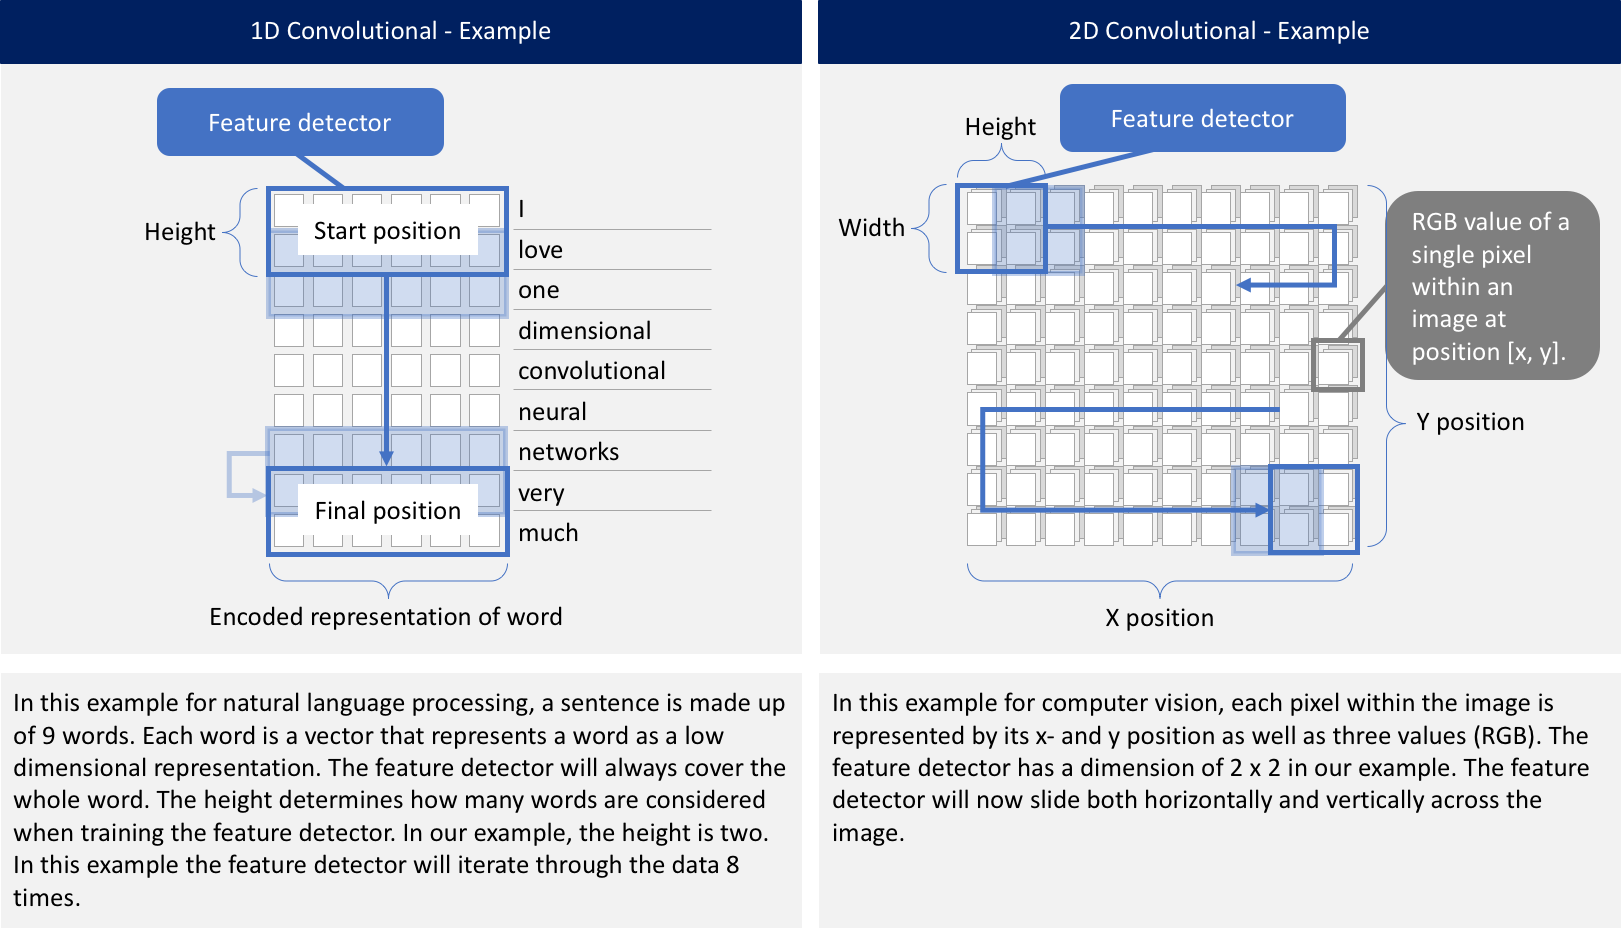
\includegraphics[scale=0.2]{conv1d}
\caption{Differenza convoluzione 1D e 2D}
\end{figure}

\section{Dataset}
Il dataset chb mit...
\todo{Provenienza, composizione, preprocessing}

\section{Backend}
L'applicazione è strutturata come una web application. La parte di backend è utilizzabile indipendentemente dall'interfaccia fornita. 
\subsection{Django Framework}
Per la realizzazione della web app abbiamo fatto uso del framework Django. Si traatta di un web frameworke di alto livello scritto in linguaggio Python, sviluppato dalla Django Software Foundation e distribuito open source. Django fa uso del paradigma Model-Template-View. 
\begin{itemize}
\item Model: è la parte del programma che si occupa del database. Django fornisce una serie di comandi rapidi per la gestione delle operazioni più comuni.
\item Template: consiste in una serie di documenti per la generazione di codice HTML, combinando l'utilizzo di parti statiche e tag dinamici. In questo progetto non è stato tuttavia utilizzato alcun template, dato che la parte visuale è gestita esternamente dal framework Ionic. 
\item View: gestisce l'interazione tra utente, sistema e database. Si occupa di ricezione, elaborazione e risposta alle richieste dell'utente.
\end{itemize}

\subsection{Python}
La sezione di backend del programma è stata scritta in Python, linguaggio di programmazione orientato agli oggetti. Di seguito sono descritte le più importanti librerie utilizzate. 

\subsection{PyEDFlib}
Il funzionamento base del sistema prevede la lettura di tracciati EEG. Questi vengono comunemente distribuiti nel formato EDF (European Data Format), ideato per lo scambio di segnali multucanali fisici e biologici. La libreria che si occupa dell'interazione con tali file è PyEDFlib, basata a sua volta su edflib e Numpy. Essa mette a disposizione funzioni per la lettura dei segnali del file e dei suoi metadati, tra cui il numero di canali, la lunghezza e la frequenza del campionamento, l'inizio e la fine della rilevazione. 

\subsection{PyTorch}
La parte di neural network e deep learning è stata realizzata mediante l'utilizzo del framework PyTorch

\subsection{API}
L'utente ha la possibilità di interagire con il sistema attraverso richieste HTTP
\todo{views singolo file, view traininig}



\nocite{*}
\printbibliography[heading = bibintoc]
\end{document}